\section{Modeling Languages and Abstract Models}

\subsection{HDL analysis}
A language can be characterized by its  syntax, semantics  and  pragmatics.\\
The \textit{syntax} relates to the language structure and it can be specified by a grammar.\\
The \textit{semantics} relates to the meaning of a language. The semantic rules associate actions to the language fragments that satisfy the syntax rules.\\
The \textit{pragmatics} relate to the other aspects of the language, including implementation issues. \\
Languages can be broadly classified as  procedural  and  declarative  languages. \textit{Procedural} programs specify the desired action by describing a sequence of steps whose order of execution matters. Conversely, \textit{declarative} models express the problem to be solved by a set of declarations without detailing a solution method. Therefore the order of the statements is not important in such languages.\\
Languages for hardware specification are classified on the basis of the description view that they support (e.g., physical, structural or behavioral).\\
Languages that support \textit{physical design} are characterized by having geometric primitives and by supporting operations on those primitives.\\
Models in \textit{structural languages} describe an interconnection of components. Hence their expressive power is similar to that of circuit schematics, even though specific language constructs can provide more powerful abstractions. Hierarchy is often used to make the description modular and compact.\\
Type of languages:
\begin{itemize}
\item Procedural languages: Specify the action (and so the circuit) by a sequence of steps (C, Pascal, VHDL, Verilog)
\item Declarative languages: Specify the hardware by a set of declaration (Logic netlist, VHDL, Verilog).
\end{itemize}
The success of VHDL and Verilog is due to at behavioral view it possible implement \textit{sequential} and \textit{combinational} descriptions.\\
Models in \textit{behavioral languages} can describe \textit{combinational} or \textit{sequential} circuits.\\
The \textit{combinational} circuit is described as a set of untimed assignment where each assignment represents a virtual logic gate (very similar to procedural models).\\
The sequential circuit is described throw declaration of \textit{Task}, use timing annotation for delayed signals. \\
The \textit{Tasks} can be, at architectural level, generic operations, or, at logic-level, logic functions.

\subsection{Abstract models}
A  model of a circuit is an abstraction, i.e., a representation that shows relevant features without associated details. Formal models have a well-defined syntax and semantics. Hence they provide a way of conveying the information about a circuit in a consistent way that can be unambiguously interpreted. Conversely, informal circuit specifications, such as textual descriptions have limited applications when  CAD  methods are used. In addition, informal descriptions of large-scale circuits or systems may be sources of misunderstanding among humans.\\
A circuit can be modelled differently according to the desired abstraction level (e.g., architectural, logic, geometric), view (e.g., behavioral, structural, physical) and the modelling means (e.g., language, diagram, mathematical model).\\
In recent years, there has been a trend toward using \textbf{hardware description languages} (HDLs) for circuit specification.\\
\textbf{Abstract models} are mathematical models based on graphs and Boolean algebra.\\
At the \textit{architectural level}, the circuit \textit{behavior} can be abstracted by a set of operations (called also tasks) and their dependencies. The operations can be general in nature, ranging from arithmetic to logic functions.\\
At the \textit{logic level}, the \textit{behavior} of a sequential logic circuit is abstracted by a finite-state machine that degenerates to a Boolean function in the  combinational case.\\
\textit{Structural views} are abstracted as interconnections of logic blocks or gates (at the logic level) or resources (at the architectural level).\\
Abstract models are powerful enough to capture the essential features described by HDL and diagram models. 
\begin{figure}[H]
	\centering
	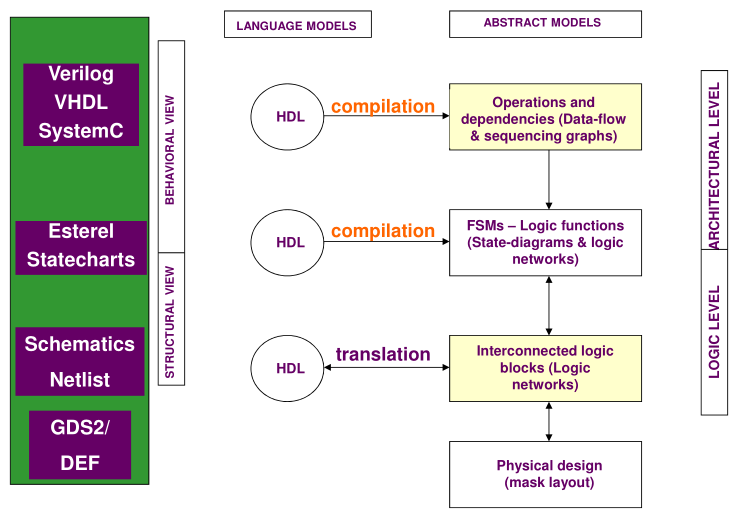
\includegraphics[height=100 mm]{./Cap2/Images/Image01.png}
	\caption[Optional caption]{Languages and abstract models}
	\label{fig:absMod}
\end{figure}
$ $\\[\spaceBreackLine]
Examples of \textbf{Abstract models}
\begin{itemize}
\item \textit{Logic networks}
\begin{itemize}
\item \textit{Mixed structural/behavioral views}
\item \textit{BDD} and \textit{AIG}
\end{itemize}
\item \textit{State diagrams}: The behavioral view of sequential circuits at the logic level can be expressed by finite-state machine transition diagrams
\item \textit{Dataflow} and \textit{sequencing graphs}
\end{itemize}

\subsubsection{Logic network (logic-level)}
A generalized \textit{logic network} is a structure, where each module is associated with a combinational or sequential logic function. Each block is modelled by a Boolean function. Each module is associated with a multiple-input, single-output combinational logic function, called a\textit{ local function}. Pins are partitioned into two classes, called \textit{input} and \textit{outputs}.
\subsubsection{Mixed structural/behavioral views}
In general, a logic network is a hybrid \textit{stmctural/behavioral representation}, because the the interconnections provide a structure while the logic functions denote the terminal behavior of the modules.
\begin{figure}[H]
    \centering
    \begin{subfigure}[b]{0.4\textwidth}
        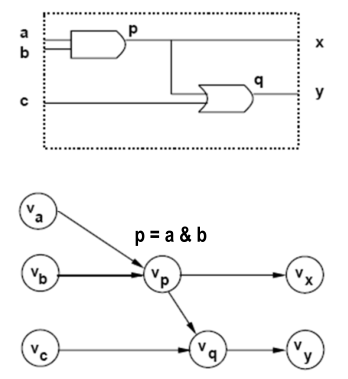
\includegraphics[width=\textwidth]{./Cap2/Images/Image02.png}
        \caption{Mapped network}
        \label{fig:map}
    \end{subfigure}
    \begin{subfigure}[b]{0.4\textwidth}
        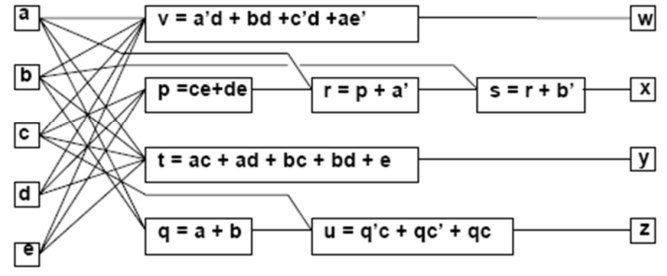
\includegraphics[width=\textwidth]{./Cap2/Images/Image03.png}
        \caption{General network}
        \label{fig:gen}
    \end{subfigure}
    \caption{Different networks}
    \label{fig:nets}
\end{figure}
The Figure \ref{fig:map} is a special case when the blocks correspond to \textit{library elements}.

\subsubsection{BDD (logic-level)}
A Binary Decision Diagram (BDD) is a directed acyclic graph (DAG)
\begin{itemize}
\item \textit{Graph}: set of vertices connected by edges
\item \textit{Directed}: edges have direction
\item \textit{Acyclic}: no path in the graph can lead to a cycle
\end{itemize}
Ordered BDD (\textbf{OBDD}):
\begin{enumerate}
\item Each vertex represents a decision on a variable
\item The value of the function is found at the leaves
\item Each path from root to leaf corresponds to a row in the truth table
\item Variables must appear in the same order along each path from root to leaves
\item Each variable can appear at most once on a path
\end{enumerate}
\begin{figure}[H]
    \centering
    \begin{subfigure}[b]{0.15\textwidth}
        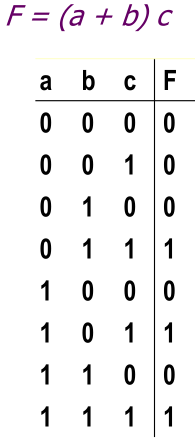
\includegraphics[width=\textwidth]{./Cap2/Images/Image04.png}
        \caption{True Table}
        \label{fig:trueTable}
    \end{subfigure}
    \quad\quad\quad
    \begin{subfigure}[b]{0.4\textwidth}
        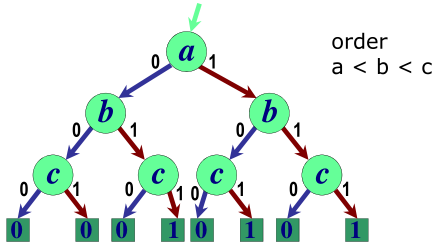
\includegraphics[width=\textwidth]{./Cap2/Images/Image05.png}
        \caption{OBDD}
        \label{fig:OBDD}
    \end{subfigure}
    \label{fig:OBDDs}
\end{figure}
The OBDD is a efficient way to represent logic functions. Each distinct function corresponds to a unique distinct diagram (\textit{Canonical form}). Efficient manipulation of Boolean functions, in fact many logical operations on OBDDs can be implemented in polynomial time (conjunction, negation, disjunction).\\
\textit{Drawbacks}: The size of a BDD is as big as a truth table.
\bigskip \\
The \textbf{Reduced OBDD} is obtained applying 2 roles:
\begin{enumerate}
\item Merging equivalent sub-trees
\item Removing nodes with identical children
\end{enumerate}

\subsubsection{AIG (logic-level)}
An And-Inverter Graph (AIG) is a  directed acyclic graph (DAG).
\textit{Nodes}:
\begin{itemize}
\item Terminal nodes representing variable names
\item Internal nodes representing AND function
\end{itemize}
\textit{Edge}: Those containing markers indicate logical negation.\\
AIG is fast, scalable (less memory) and with efficient manipulation. Each function can have different diagrams, it is not a \textit{Canonical form}.\\
The advantage of the AIG: the number of the leafs is equal to the number of the inputs (n) and not $ 2^{n} $ as in the ROBDD.
\begin{figure}[H]
	\centering
	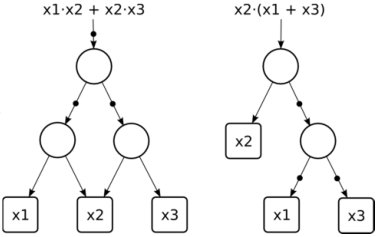
\includegraphics[height=50 mm]{./Cap2/Images/Image07.png}
	\caption[Optional caption]{Different Diagrams of the same function}
	\label{fig:aig}
\end{figure}
The Figure \ref{fig:aig} shows the AIG diagrams. Them must be read from the bottom to up.\\
Remember the \textit{Morgan's law}: $ \overline{x_{1} + x_{2}} = \overline{x_{1}} \overline{x_{2}} $\\
In the first diagram: $ \overline{\overline{x_{1} x_{2}} \, \overline{x_{2} x_{3}}} = x_{1} x_{2} + x_{2} x_{3} $

\subsubsection{State  Diagrams}
The behavioral view of sequential circuits at the logic level can be expressed by finite-state machine transition diagrams. A finite-state machine can be described by:
\begin{itemize}
\item A set of primary input panems, $X$
\item A set of primary output patterns, $Y$
\item A set of states, $S$
\item A \textit{state transition} function, $\delta : X \times S \rightarrow S$
\item An \textit{output function},  $\lambda :  X \times S \rightarrow Y $ for \textit{Mealy} models or  $\lambda : S \rightarrow Y $ for \textit{Moore}
\item An initial state
\end{itemize}
The \textit{state transition table} is a tabulation of the state transition and output functions. Its corresponding graph-based representation is the \textit{state transition diagram}.
\begin{figure}[H]
	\centering
	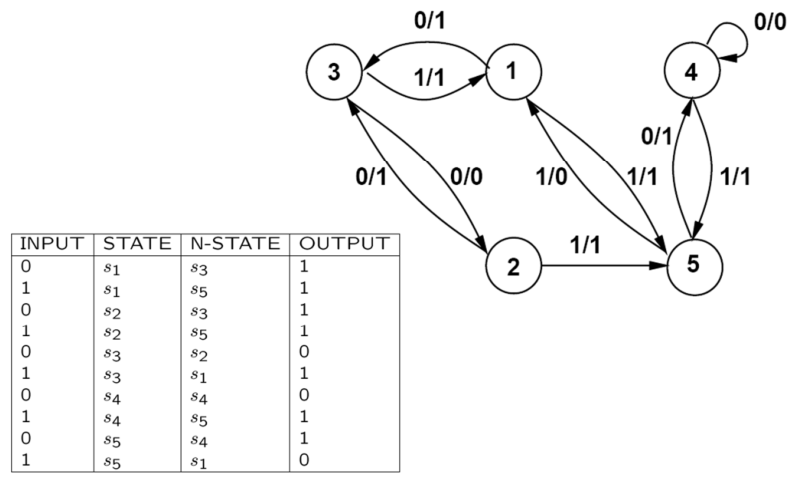
\includegraphics[height=45 mm]{./Cap2/Images/Image06.png}
	\caption[Optional caption]{State transition table and state transition diagram}
	\label{fig:stateDia}
\end{figure}

\subsubsection{Dataflow graphs – DFG (Architectural-level)}
We consider here models that abstract the information represented by procedural HDLs. Abstract models of behavior at the architectural level are in terms of  \textit{operations}  (Vertices)  and their  \textit{dependencies} (Edges).
\begin{figure}[H]
	\centering
	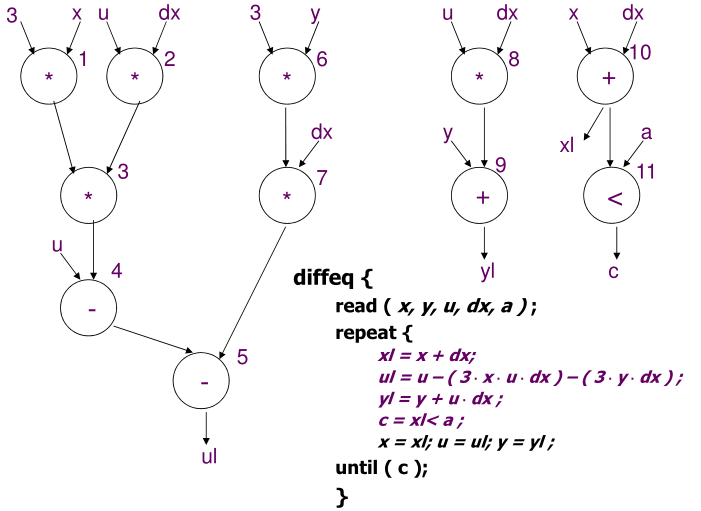
\includegraphics[height=45 mm]{./Cap2/Images/Image08.png}
	\caption[Optional caption]{DFG}
	\label{fig:DFG}
\end{figure}
Control-flow information, related to  \textit{branching}  (or  \textit{conditional})  and  \textit{iteration} (or  \textit{loop})  constructs, can also be represented graphically. Many different models have been proposed to represent \textit{control/data-flow graphs}.\\
The simplest approach is to extend further data-flow graphs by introducing branching vertices that represent operations that evaluate conditional clauses.  A  \textit{branching} vertex is the tail of a set of alternative paths, corresponding to the possible branches. \textit{Iteration} can be modelled as a branch based on the iteration exit condition. The corresponding vertex is the tail of two edges, one modelling the exit from the loop and the other the return to the first operation in the loop.\\
One particular abstract model for tasks subject to data- and control-flow dependencies is called \textit{sequencing graph}. It is a hierarchical control/data-flow graph, where control-flow primitives such as branching and iteration are modelled through the hierarchy, whereas data-flow and serialization dependencies are modelled by graphs. In addition, the hierarchical model supports a  model call,  i.e., the encapsulation of subsets of operations and their dependencies into blocks that can be multiply invoked.\\
The graph has two major properties:
\begin{itemize}
\item Acyclic
\item Polar: there are two vertices, called  \textit{source}  and  \textit{sink},  that represent the first and last tasks.
\end{itemize}
\begin{figure}[H]
    \centering
    \begin{subfigure}[b]{0.2\textwidth}
        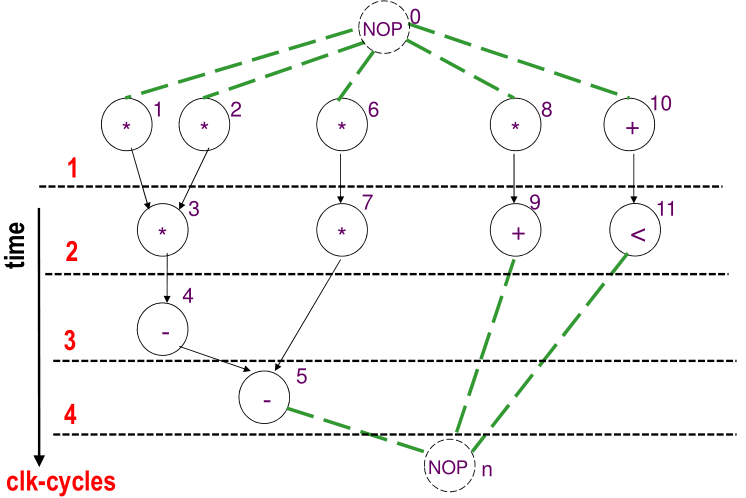
\includegraphics[width=\textwidth]{./Cap2/Images/Image09.png}
        \caption{Sequencing DFG}
        \label{fig:SequencingDFG}
    \end{subfigure}
    \quad
    \begin{subfigure}[b]{0.2\textwidth}
        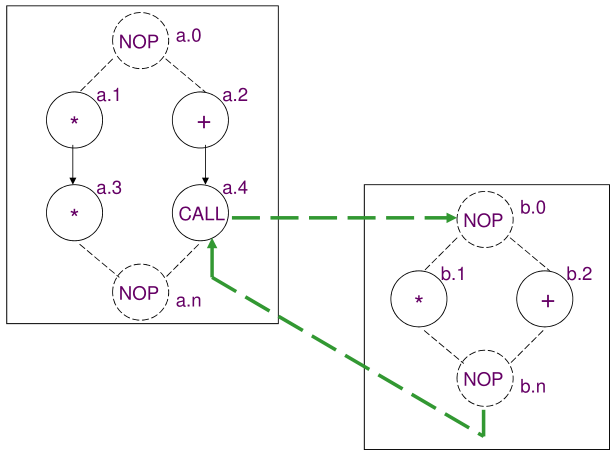
\includegraphics[width=\textwidth]{./Cap2/Images/Image10.png}
        \caption{Hierarchy DFG}
        \label{fig:HierarchyDFG}
    \end{subfigure}
    \quad
    \begin{subfigure}[b]{0.2\textwidth}
        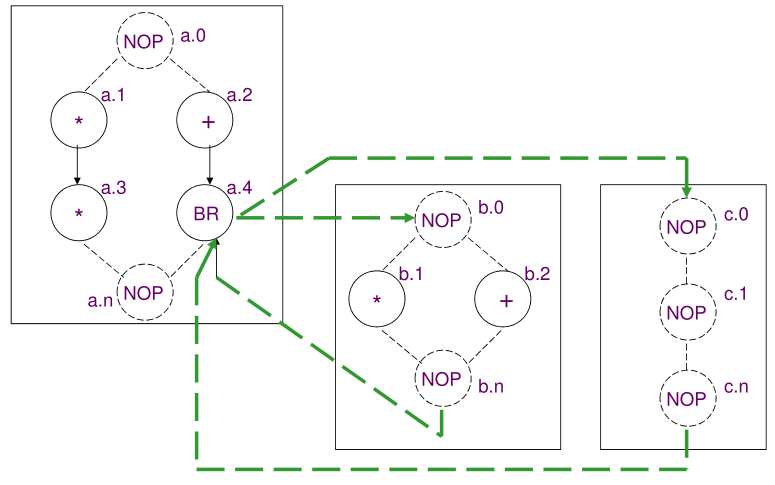
\includegraphics[width=\textwidth]{./Cap2/Images/Image11.png}
        \caption{Branching DFG}
        \label{fig:BranchingDFG}
    \end{subfigure}
    \quad
    \begin{subfigure}[b]{0.2\textwidth}
        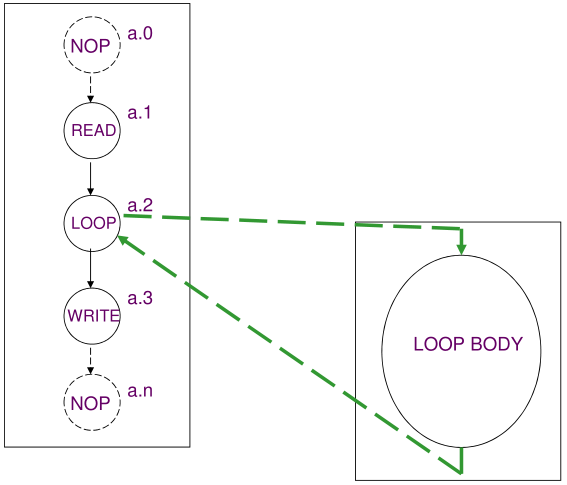
\includegraphics[width=\textwidth]{./Cap2/Images/Image12.png}
        \caption{Iteration DFG}
        \label{fig:IterationDFG}
    \end{subfigure}
    \label{fig:DFGs}
    \caption{Different examples of DFG}
\end{figure}
Some attributes can be assigned to the vertices and edges of a sequencing graph model, such as measures or estimates of the corresponding \textit{area} or delay \textit{cost}. In general, the delay of  a  vertex can be  data independent  or  data dependent.  Only data-independent delays can be estimated before synthesis. An example data-dependent iteration is given by an arithmetic divisor, based on an iterative algorithm. Data-dependent delays can be  \textit{bounded}  or  \textit{unbounded}.  The former case applies to data-dependent delay branching, where the maximum and minimum possible delays can be computed. The latter case is typical of some other iteration constructs.